\section{Goal and Scope}
\label{section:goal_and_scope}

The goal of this project is to develop a user-friendly application that can generate modern 3D cities and export them in a standard 3D file format such as \textit{.fbx}.
\textit{User-friendly} denotes that users should not need any technical expertise or coding experience to fully utilize the application.
Furthermore, \textit{modern cities} will be defined as cities that resemble present industrialized cities such as New York, Paris, San Francisco, and Tokyo (see Figure~\ref{fig:ModernCities}).
The intention is not to perfectly replicate these cities, but rather to draw inspiration from them.

\begin{figure}[h!]
  \centering

  \begin{subfigure}[b]{0.56\textwidth}
    \frame{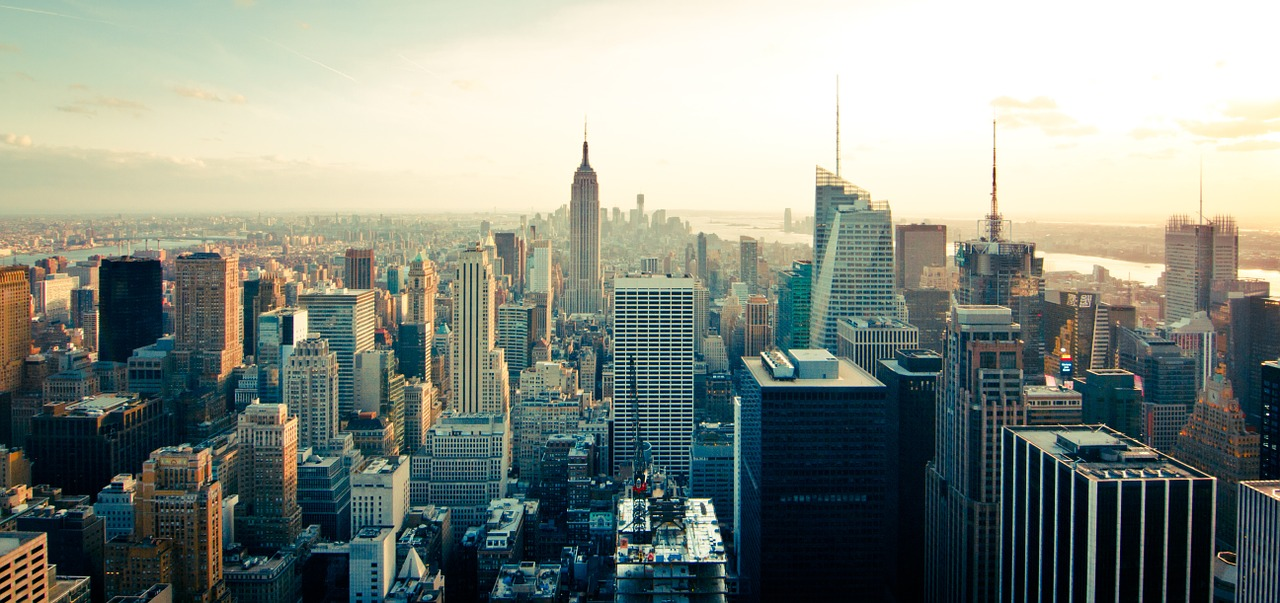
\includegraphics[width=\textwidth]{figure/modern-city-manhattan.jpg}}
    \caption{Manhattan, New York \cite{manhattan_img}.}
  \end{subfigure}
  \quad
  \begin{subfigure}[b]{0.395\textwidth}
    \frame{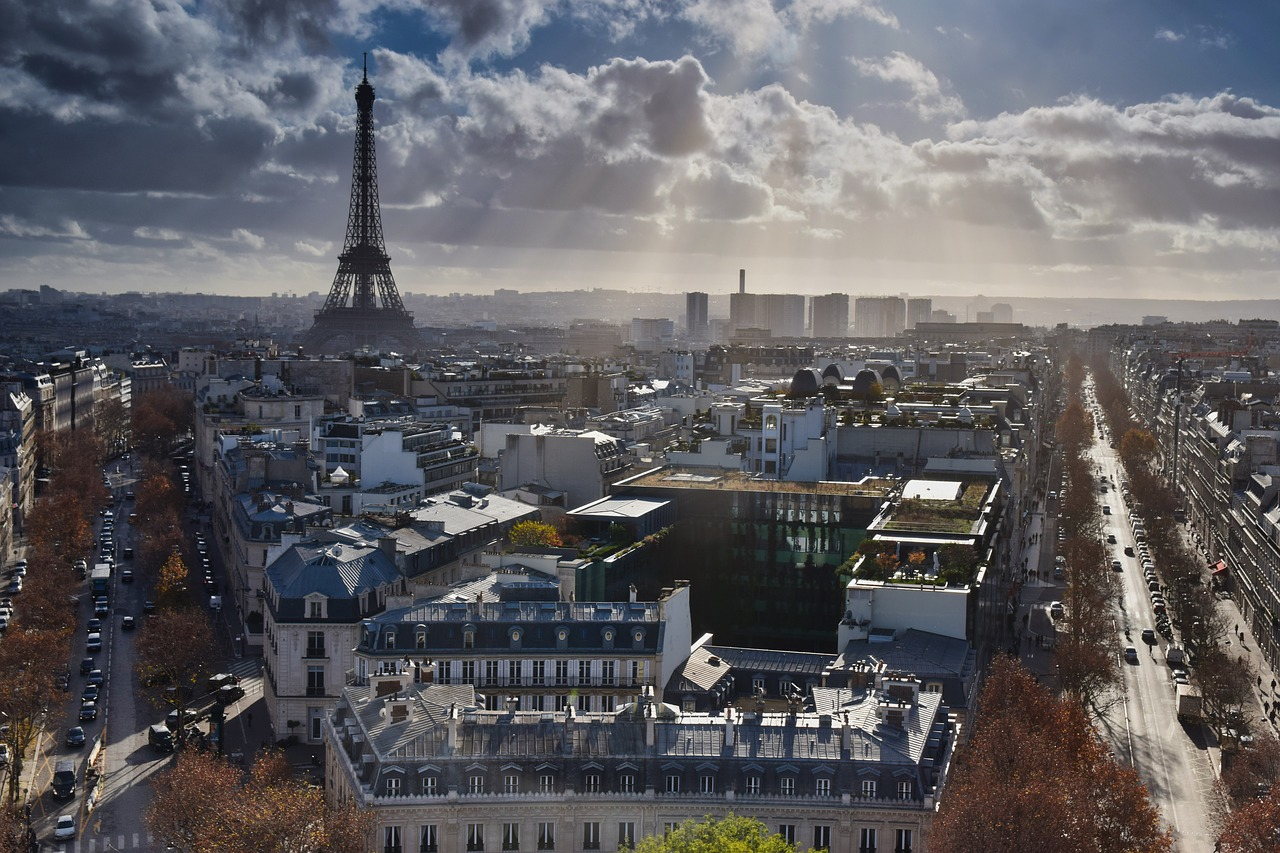
\includegraphics[width=\textwidth]{figure/modern-city-paris.jpg}}
    \caption{Paris \cite{paris_img}.}
  \end{subfigure}

  \caption{Two examples of modern cities considered in this project.}
  \label{fig:ModernCities}
\end{figure}

To clarify, suburban and rural areas are also included as part of such modern cities.

The process of generating cities should be effortless both in the sense that minimal configuration should be required, and that generation of multiple cities should be feasible within a minute from application start when running on a modern laptop.
With that said, the visual quality of models is not of immediate concern for this work.
The intention is to demonstrate a proof of concept of how PCG algorithms can be used to leverage the effort required to build cities, not to produce production-ready software.
Consequently, the use of free textures and models is encouraged in order to prioritize the development of algorithms.
Additionally, any specific art style such as low poly \cite{lowpoly_wiki} and voxel graphics \cite{voxels_wiki} is not pursued.

The generation of roads and buildings will be of primary focus, as these are considered the core features of a city.
Surrounding terrain also needs to be generated, mainly to form natural settings which the city infrastructures need to adjust after.
Accordingly, the terrain itself does not need any significant level of detail.
Other metropolis aspects such as sidewalks, parks and parking lots are also intended to be generated, albeit with less variation.

In this contribution, generated cities will be restricted to static models in order to support integration with a wider array of third-party software.
Therefore, dynamic content such as simulation of road traffic, day-night cycles, and pedestrians are all considered out of scope.
The interior of buildings is also considered out of scope since end-users are expected to desire more control over such content than what this project's time frame can support.

As a consequence of the random and visual aspects of PCG, it is difficult to express a precise definition that can measure whether this project's final results should be considered successful or not.
Nevertheless, the following list has been constructed as a modest checklist to capture and discuss the quality of the resulting application.

\vspace{-0.5cm} % match spacing of easylist
\begin{itemize}
  \item[\textbf{Q1:}] Do models correctly integrate with third-party software such as Blender \cite{blender}?
  \item[\textbf{Q2:}] How well is the codebase structured for replacement and expansion of features?
  \item[\textbf{Q3:}] How much notable variety is there in the generated content?
  \item[\textbf{Q4:}] To what degree do the generated cities resemble real-world cities?
  \item[\textbf{Q5}:] How much control do the users have over the generation?
  \item[\textbf{Q6}:] Are the cities suitable for use in digital media such as games and film?
  \item[\textbf{Q7}:] Are users without technical expertise able to correctly use the application?
  \item[\textbf{Q8}:] Are there any known bugs or crashes in the application, or any visual artifacts in the generated models?
\end{itemize}
